\section{IBM Company Technology Innovation Strategy}

IBM is one of the world's leading technology companies, with a long history of innovation. The company's technology innovation strategy is focused on five key areas: hybrid cloud, artificial intelligence (AI), quantum computing, systems and semiconductors, and security.
\begin{enumerate}


    \item \textbf{Hybrid Cloud} IBM is a leader in hybrid cloud computing, which combines the flexibility and scalability of public cloud with the security and control of private cloud. IBM's hybrid cloud solutions are designed to help businesses of all sizes modernize their IT infrastructure, improve their efficiency, and reduce their costs.

    \item \textbf{Artificial Intelligence} IBM is also a leader in AI, which is rapidly transforming the way businesses operate. IBM's AI solutions are designed to help businesses automate tasks, improve decision-making, and create new products and services.

    \item \textbf{Quantum Computing}

IBM is at the forefront of quantum computing, which has the potential to revolutionize many industries. IBM's quantum computing solutions are designed to help businesses solve complex problems that are intractable with traditional computers.

    \item \textbf{Systems and Semiconductors}

IBM is also a leader in systems and semiconductors, which are the critical components of modern technology infrastructure. IBM's systems and semiconductor technologies are designed to help businesses build and operate high-performance, reliable, and secure IT systems.

    \item \textbf{Security}

Security is another key focus area for IBM's technology innovation strategy. IBM's security solutions are designed to help businesses protect their data and systems from cyberattacks.
\end{enumerate}

IBM's technology innovation strategy is driven by a deep understanding of customer needs and the challenges they face. The company invests heavily in research and development, and it has a large network of research labs around the world. IBM also collaborates with partners from academia, industry, and government to develop innovative solutions.


Here are some specific examples of IBM's technology innovation:

\begin{itemize}
  \item IBM Cloud Paks are integrated software solutions that combine IBM software with Red Hat OpenShift to help businesses deploy and manage applications in hybrid and multi-cloud environments.
  \item IBM Watson AI is a cognitive computing platform that helps businesses automate tasks, improve decision-making, and create new products and services.
  \item IBM Quantum System One is the first commercially available quantum computer.
  \item IBM POWER10 is a high-performance processor that is used in IBM's servers and mainframes.
  \item IBM Z16 is a high-performance mainframe that is designed to handle demanding workloads such as transaction processing and analytics.
  \item IBM Security QRadar is a security information and event management (SIEM) platform that helps businesses detect and respond to cyberattacks.
\end{itemize}

IBM's technology innovation strategy is helping the company to remain a leader in the technology industry. The company's focus on hybrid cloud, AI, quantum computing, systems and semiconductors, and security is well-aligned with the key trends that are shaping the future of technology.

\subsection{Impact of IBM's Technology Innovation Strategy}

IBM's technology innovation strategy is having a significant impact on its customers and the industries it serves. For example, IBM's hybrid cloud solutions are helping businesses to modernize their IT infrastructure, improve their efficiency, and reduce their costs. IBM's AI solutions are helping businesses to automate tasks, improve decision-making, and create new products and services. IBM's quantum computing solutions are helping businesses to solve complex problems that are intractable with traditional computers. IBM's systems and semiconductor technologies are helping businesses to build and operate high-performance, reliable, and secure IT systems. IBM's security solutions are helping businesses to protect their data and systems from cyberattacks.

Overall, IBM's technology innovation strategy is helping the company to make a positive impact on the world. IBM's technologies are helping businesses to improve their operations, create new products and services, and solve complex problems. IBM's technologies are also helping to make the world a safer place by protecting businesses from cyberattacks.

\subsection{IBM's Patent Trends}
IBM, or International Business Machines Corporation, has a long history of innovation and a significant presence in the field of patents. As of my last knowledge update in January 2022, IBM was consistently one of the top patent-holding companies globally. Here are some key points about IBM's patent trends:


\begin{itemize}
  \item \textbf{Consistent Patent Leader:} IBM has consistently ranked as one of the top patent-holding companies globally. They often compete with other technology giants like Samsung, Canon, and Microsoft for the top spot.

  \item \textbf{Diverse Patent Portfolio:} IBM's patent portfolio covers a wide range of technology areas, including artificial intelligence, cloud computing, cybersecurity, data analytics, and quantum computing. They are known for their strong focus on emerging technologies.

  \item \textbf{Strategic Investments:} IBM has made strategic investments in research and development, contributing to its robust patent portfolio. They have research labs and facilities around the world, where scientists and engineers work on cutting-edge technologies.

  \item \textbf{Quantum Computing:} IBM is a notable player in the field of quantum computing, and they have also secured patents related to quantum computing technologies.

  \item \textbf{Open Innovation:} IBM has a history of participating in open-source projects and initiatives, which can sometimes lead to patent-related considerations in the open-source community.

  \item \textbf{Licensing and Revenue:} IBM not only uses its patents for internal purposes but also licenses its intellectual property to other companies. This can generate significant revenue for the company.
\end{itemize}

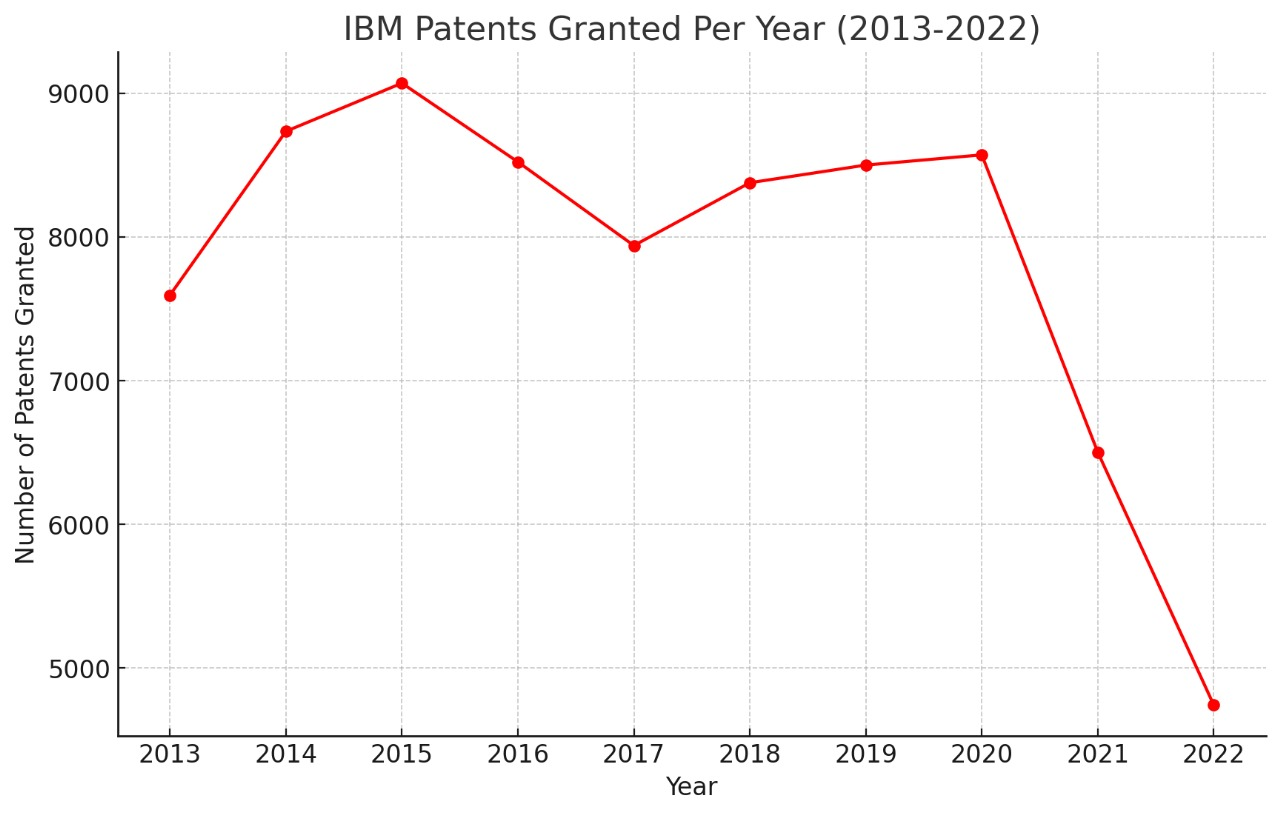
\includegraphics[width=\textwidth]{image}

Here is the graph depicting the number of patents granted to IBM each year from 2013 to 2022, based on the data you provided. The graph shows variations in the number of patents granted over this period, with a general trend of increase until around 2020, followed by a decrease in the last two years.

\subsection{Factors Contributing to Decline in IBM's Patent Grants}

The decline in the number of patents granted to IBM in subsequent years could be attributed to several factors:

\begin{itemize}
  \item \textbf{Strategic Shift in Innovation Focus:} Companies often shift their strategic focus over time, which can affect their patent output. IBM has been known to realign its research and development efforts towards new and emerging fields like artificial intelligence, quantum computing, and cloud services. This shift might lead to a decrease in the quantity of patents but potentially an increase in their strategic importance or quality.

  \item \textbf{Changes in Patent Filing Strategies:} The approach to patenting can change over time, prioritizing quality over quantity. IBM might have decided to pursue fewer, more impactful patents rather than a larger number of broad, less significant ones.

  \item \textbf{Market and Technological Changes:} As technology and market demands evolve, IBM's research and development efforts might also adapt, potentially leading to a temporary decrease in patent output as new areas of research are developed.

  \item \textbf{Economic and Budgetary Considerations:} Economic factors, including R\&D budgets and cost considerations, can influence the number of patents a company files. Reducing expenses in certain areas can lead to fewer patent filings.

  \item \textbf{Competitive Landscape:} The rise of new competitors in key technology areas can also influence patent counts. As more companies enter fields like AI and cloud computing, IBM's relative share of patents in these areas might decrease.
\end{itemize}

It's important to note that a decrease in patent numbers doesn't necessarily reflect a decline in innovation or success. Companies like IBM often focus on the strategic value of patents, which isn't solely determined by quantity.



\subsection{IBM's Approach to Innovation and R\&D}

IBM's approach to innovation and R\&D is centered on three key pillars:

\begin{enumerate}
  \item \textbf{Deep Understanding of Customer Needs and Challenges:} IBM researchers work closely with customers to understand their needs and the challenges they face. This helps IBM to identify the most important areas to invest in and to develop solutions that are truly relevant to customers.
  
  \item \textbf{Investment in Fundamental Research:} IBM invests heavily in fundamental research, which is the exploration of new ideas and concepts without a specific application in mind. This investment is essential for developing the breakthrough technologies that will drive innovation in the future.
  
  \item \textbf{Collaboration:} IBM collaborates with partners from academia, industry, and government to develop innovative solutions. This collaboration allows IBM to leverage the expertise of others and to bring new technologies to market more quickly.
\end{enumerate}

IBM's approach to innovation and R\&D has been successful in delivering groundbreaking technologies that have transformed many industries. For example, IBM researchers developed the first mainframe computer, the first personal computer, and the first commercial quantum computer. IBM's researchers are also at the forefront of other emerging technologies such as artificial intelligence, blockchain, and the Internet of Things.

Here are some specific examples of IBM's approach to innovation and R\&D:

\begin{itemize}
  \item IBM has a network of research labs around the world, where researchers are working on a wide range of cutting-edge technologies.
  \item IBM invests heavily in open source software, which allows it to collaborate with a global community of developers on new ideas.
  \item IBM has a number of venture capital funds that invest in early-stage startups developing innovative technologies.
  \item IBM partners with universities and other research institutions to conduct joint research projects.
  \item IBM works with government agencies to develop and deploy new technologies that can address societal challenges.
\end{itemize}

IBM's approach to innovation and R\&D is essential to the company's continued success in a rapidly changing technological landscape. By investing in fundamental research, collaborating with others, and understanding the needs of its customers, IBM is able to develop the technologies that will drive the future.

\subsection{IBM's Investment in Research and Development (R\&D)}

IBM is one of the world's leading investors in research and development (R\&D). In 2022, IBM spent \$6.57 billion on R\&D, which accounted for approximately 6.5\% of its revenue. This is significantly higher than the average R\&D investment as a percentage of revenue for the global technology industry, which is around 3\%.

IBM's investment in R\&D is focused on five key areas: hybrid cloud, artificial intelligence (AI), quantum computing, systems and semiconductors, and security. These are the areas where IBM believes that the most important technological breakthroughs will occur in the years to come.

IBM's investment in R\&D has paid off in a number of ways. IBM has developed some of the world's most innovative technologies, including the mainframe computer, the personal computer, and the commercial quantum computer. IBM's R\&D has also led to the development of many other important technologies, such as disk drives, ATMs, and artificial intelligence algorithms.

IBM's investment in R\&D is also beneficial to the broader economy. IBM's research labs employ thousands of scientists and engineers, and they help to train the next generation of technology leaders. IBM's R\&D also leads to the development of new products and services that can create jobs and boost economic growth.

Here are some specific examples of how IBM's investment in R\&D is benefiting the company and the economy:

\begin{itemize}
  \item IBM's research on hybrid cloud computing is helping businesses to modernize their IT infrastructure, improve their efficiency, and reduce their costs.
  \item IBM's research on AI is helping businesses to automate tasks, improve decision-making, and create new products and services.
  \item IBM's research on quantum computing is helping businesses to solve complex problems that are intractable with traditional computers.
  \item IBM's research on systems and semiconductors is helping businesses to build and operate high-performance, reliable, and secure IT systems.
  \item IBM's research on security is helping businesses to protect their data and systems from cyberattacks.
\end{itemize}

IBM's investment in R\&D is essential to the company's continued success in a rapidly changing technological landscape. By investing in R\&D, IBM is able to develop the technologies that will drive the future and create value for its customers, shareholders, and employees.

\subsection{IBM's Collaborations and Partnerships in the Technology Space}

IBM collaborates with a wide range of partners in the technology space, including universities, research institutions, startups, and other technology companies. These partnerships allow IBM to leverage the expertise of others, accelerate the development of new technologies, and bring these technologies to market more quickly.

\subsubsection{Specific Examples of Collaborations and Partnerships}

Here are some specific examples of IBM's collaborations and partnerships in the technology space:

\begin{itemize}
  \item \textbf{Universities and Research Institutions:} IBM has joint research agreements with many leading universities and research institutions around the world. These partnerships allow IBM researchers to collaborate with their peers on new technologies and to access cutting-edge research facilities. For example, IBM has a joint research agreement with MIT on artificial intelligence, and it has a joint research agreement with Stanford University on quantum computing.
  
  \item \textbf{Startups:} IBM invests in and partners with startups developing innovative technologies. This allows IBM to stay ahead of the curve and to bring new technologies to market quickly. For example, IBM has invested in startups developing new cloud computing technologies, artificial intelligence technologies, and cybersecurity technologies.
  
  \item \textbf{Other Technology Companies:} IBM also partners with other technology companies to develop and deploy new technologies. For example, IBM has a partnership with Samsung to develop new semiconductor technologies, and it has a partnership with Adobe to develop new customer experience solutions.
\end{itemize}

\subsubsection{Benefits of Collaborations and Partnerships}

IBM's collaborations and partnerships in the technology space are essential to the company's continued success. By working with others, IBM is able to develop new technologies more quickly and efficiently, and it is able to bring these technologies to market more effectively.

Here are some of the benefits of IBM's collaborations and partnerships in the technology space:

\begin{itemize}
  \item \textbf{Accelerated Innovation:} By collaborating with others, IBM is able to accelerate the development of new technologies. This is because IBM can leverage the expertise of its partners and access their resources. For example, IBM's partnership with MIT on artificial intelligence has helped to accelerate the development of new AI technologies.
  
  \item \textbf{Reduced Costs:} Collaborating with others can also help IBM to reduce the costs of developing and deploying new technologies. This is because IBM can share the costs with its partners. For example, IBM's partnership with Samsung on semiconductor technologies has helped to reduce the costs of developing new chip designs.
  
  \item \textbf{Increased Market Share:} IBM's collaborations and partnerships can also help the company to increase its market share. This is because IBM can gain access to new markets through its partners. For example, IBM's partnership with Adobe on customer experience solutions has helped IBM to increase its market share in the customer experience market.
\end{itemize}

Overall, IBM's collaborations and partnerships in the technology space are essential to the company's continued success. By working with others, IBM is able to develop and deploy new technologies more quickly, efficiently, and effectively.


\section{Customer Orientation of IBM}

IBM is a customer-oriented company. This means that IBM puts its customers' needs and wants first in everything it does. IBM's customer orientation is evident in its product development, sales and marketing, and customer support efforts.
\begin{enumerate}
\item \textbf{Product Development}

IBM's product development process is centered on understanding and meeting the needs of its customers. IBM researchers and product developers work closely with customers to understand their pain points and to develop solutions that address those pain points. IBM also uses customer feedback to improve its existing products and services.

For example, IBM's Watson AI platform was developed in response to customer demand for a cognitive computing platform that could help businesses to automate tasks, improve decision-making, and create new products and services. IBM's Cloud Paks were also developed in response to customer demand for a hybrid cloud solution that could help businesses to modernize their IT infrastructure, improve their efficiency, and reduce their costs.

\item \textbf{Sales and Marketing}

IBM's sales and marketing efforts are also focused on meeting the needs of its customers. IBM's sales representatives work with customers to understand their specific needs and to develop solutions that meet those needs. IBM's marketing campaigns are also designed to highlight the benefits of IBM's products and services to customers.

For example, IBM's "Let's Build a Smarter Planet" campaign highlights the benefits of IBM's technologies for helping businesses and governments to solve complex problems. IBM's "Call for Code" initiative challenges developers to create solutions that address social challenges using IBM's technologies.

\item \textbf{Customer Support}

IBM is also committed to providing excellent customer support. IBM offers a variety of customer support options, including phone support, email support, and online support. IBM also has a team of customer support experts who are available to help customers with complex problems.

For example, IBM's Global Technology Services (GTS) organization provides a wide range of IT support services to businesses around the world. IBM's GTS organization can help businesses with everything from IT consulting to managed services.
\end{enumerate}

\subsubsection{Examples of IBM's Customer Orientation}

Here are some specific examples of IBM's customer orientation:

\begin{itemize}
  \item IBM worked with customers to develop its Watson AI platform. Watson was designed to help businesses automate tasks, improve decision-making, and create new products and services.
  \item IBM worked with customers to develop its Cloud Paks. Cloud Paks are hybrid cloud solutions that can help businesses to modernize their IT infrastructure, improve their efficiency, and reduce their costs.
  \item IBM's "Let's Build a Smarter Planet" campaign highlights the benefits of IBM's technologies for helping businesses and governments to solve complex problems.
  \item IBM's "Call for Code" initiative challenges developers to create solutions that address social challenges using IBM's technologies.
  \item IBM's Global Technology Services (GTS) organization provides a wide range of IT support services to businesses around the world.
\end{itemize}

\subsubsection{Benefits of IBM's Customer Orientation}

IBM's customer orientation has a number of benefits for the company. By putting its customers' needs first, IBM is able to develop products and services that are relevant to its customers and that meet their needs. IBM is also able to build strong relationships with its customers, which can lead to repeat business and referrals.

In addition, IBM's customer orientation helps the company to stay ahead of the competition. By understanding and meeting the needs of its customers, IBM is able to identify and address new opportunities. IBM is also able to develop new products and services that meet the evolving needs of its customers.

\subsection{IBM's Focus on Customer Needs and Preferences}

IBM's focus on customer needs and preferences is evident in all aspects of its business. From product development to sales and marketing to customer support, IBM is committed to providing its customers with the best possible experience.

\subsubsection{Customer Research}

One way that IBM focuses on customer needs is by conducting extensive customer research. IBM surveys its customers regularly to understand their pain points and their needs for new products and services. IBM also has a team of customer researchers who work closely with customers to understand their businesses and their challenges.

This customer research informs IBM's product development process. IBM's product developers work closely with customers to ensure that the products they are developing meet the needs of the market. IBM also uses customer feedback to improve its existing products and services.

\subsubsection{Sales and Marketing}

IBM's sales and marketing efforts are also focused on meeting the needs of its customers. IBM's sales representatives work with customers to understand their specific needs and to develop solutions that meet those needs. IBM's marketing campaigns are also designed to highlight the benefits of IBM's products and services to customers.

For example, IBM's "Let's Build a Smarter Planet" campaign highlights the benefits of IBM's technologies for helping businesses and governments to solve complex problems. IBM's "Call for Code" initiative challenges developers to create solutions that address social challenges using IBM's technologies.

\subsubsection{Customer Support}

IBM is also committed to providing excellent customer support. IBM offers a variety of customer support options, including phone support, email support, and online support. IBM also has a team of customer support experts who are available to help customers with complex problems.

For example, IBM's Global Technology Services (GTS) organization provides a wide range of IT support services to businesses around the world. IBM's GTS organization can help businesses with everything from IT consulting to managed services.

\subsubsection{Benefits of IBM's Focus on Customer Needs and Preferences}

IBM's focus on customer needs and preferences has helped the company to become one of the world's leading technology companies. IBM's customers trust IBM to provide them with the products and services they need to succeed.

Here are some of the benefits of IBM's focus on customer needs and preferences:

\begin{itemize}
  \item \textbf{Increased Customer Satisfaction:} By focusing on customer needs and preferences, IBM is able to develop products and services that meet the needs of its customers. This leads to increased customer satisfaction and loyalty.
  
  \item \textbf{Increased Sales and Revenue:} Customer satisfaction leads to increased sales and revenue. Customers who are satisfied with IBM's products and services are more likely to continue doing business with IBM and to recommend IBM to others.
  
  \item \textbf{Competitive Advantage:} IBM's focus on customer needs and preferences gives it a competitive advantage over other technology companies. IBM is able to develop and market products and services that are more relevant to its customers' needs.
\end{itemize}

Overall, IBM's focus on customer needs and preferences is essential to the company's success. By putting its customers first, IBM is able to develop products and services that meet the needs of the market, increase customer satisfaction, and achieve a competitive advantage.


\subsection{IBM's Customer-Centric Initiatives and Feedback Mechanisms}

IBM has a number of customer-centric initiatives and feedback mechanisms in place to ensure that its products and services meet the needs of its customers.

\subsubsection{Customer-Centric Initiatives}

Some of IBM's customer-centric initiatives include:

\begin{itemize}
  \item \textbf{Client Advisory Boards (CABs):} CABs are groups of customers who provide IBM with feedback on its products and services. CAB members also help IBM to identify new opportunities and to develop new products and services.
  
  \item \textbf{Client Advocacy Program:} The Client Advocacy Program is a program that helps IBM to understand and meet the needs of its customers. The program provides IBM with direct access to its customers and allows IBM to collect customer feedback on its products and services.
  
  \item \textbf{Executive Client Dialogues:} Executive Client Dialogues are meetings between IBM executives and IBM customers. These meetings provide IBM executives with an opportunity to hear directly from IBM customers and to learn about their needs and challenges.
  
  \item \textbf{Customer Success Managers:} Customer Success Managers are IBM employees who are responsible for helping IBM customers to succeed with IBM's products and services. Customer Success Managers work closely with customers to understand their needs and to develop solutions that meet those needs.
\end{itemize}

\subsubsection{Feedback Mechanisms}

IBM has a number of feedback mechanisms in place to collect feedback from its customers. These feedback mechanisms include:

\begin{itemize}
  \item \textbf{Customer Satisfaction Surveys:} IBM surveys its customers regularly to understand their satisfaction with IBM's products and services. IBM also uses customer satisfaction surveys to identify areas where it can improve.
  
  \item \textbf{Product Feedback Surveys:} IBM also surveys its customers to collect feedback on its specific products and services. IBM uses this feedback to improve its existing products and services and to develop new products and services.
  
  \item \textbf{Customer Support Tickets:} IBM customers can submit customer support tickets to report problems with IBM's products and services. IBM uses customer support tickets to identify and resolve customer problems.
  
  \item \textbf{Social Media:} IBM also collects customer feedback through social media. IBM monitors social media platforms such as Twitter and Facebook to see what customers are saying about IBM's products and services. IBM also uses social media to respond to customer feedback and to provide customer support.
\end{itemize}

IBM takes customer feedback very seriously. IBM uses customer feedback to improve its products and services and to make sure that it is meeting the needs of its customers.

\subsubsection{Examples of Using Customer Feedback}

Here are some examples of how IBM has used customer feedback to improve its products and services:

\begin{itemize}
  \item IBM used customer feedback to improve its Watson AI platform. IBM customers wanted IBM to make Watson AI more accessible and easier to use. IBM responded to this feedback by developing Watson APIs and Watson Assistant.
  
  \item IBM used customer feedback to improve its Cloud Paks. IBM customers wanted IBM to make Cloud Paks more flexible and customizable. IBM responded to this feedback by developing new Cloud Paks and by making it easier for customers to create their own Cloud Paks.
  
  \item IBM used customer feedback to improve its customer support. IBM customers wanted IBM to provide more self-service support options. IBM responded to this feedback by developing new knowledge bases and by making it easier for customers to submit customer support tickets.
\end{itemize}

IBM's customer-centric initiatives and feedback mechanisms have helped the company to become one of the world's leading technology companies. IBM's customers appreciate IBM's commitment to understanding and meeting their needs.

\subsection{Case Studies and Examples of IBM's Customer-Oriented Strategies}

\subsubsection{Case Study 1: IBM helps ANZ Bank to Improve Customer Experience}

ANZ Bank is one of the largest banks in Australia and New Zealand. ANZ Bank faced challenges, including increasing customer churn and a complex IT infrastructure. ANZ Bank sought help from IBM.

IBM worked with ANZ Bank to develop a new customer relationship management (CRM) system. The new CRM system allowed ANZ Bank to better understand its customers and provide them with more personalized service. IBM also assisted ANZ Bank in simplifying its IT infrastructure and reducing costs.

As a result, ANZ Bank improved its customer experience, reduced customer churn, and achieved cost savings.

\subsubsection{Case Study 2: IBM helps Medtronic to Improve Patient Care}

Medtronic is a global leader in medical technology and was grappling with challenges such as rising healthcare costs and complex regulatory requirements. Medtronic turned to IBM for assistance.

IBM collaborated with Medtronic to create a new cloud-based healthcare platform. This platform helped Medtronic enhance patient care and reduce healthcare costs. IBM also aided Medtronic in complying with intricate regulatory requirements.

As a result, Medtronic improved patient care, reduced healthcare costs, and realized IT cost savings.

\subsubsection{Example 1: IBM Watson AI helps Improve Cancer Diagnosis}

IBM Watson AI is a cognitive computing platform that assists businesses in automating tasks, enhancing decision-making, and creating new products and services. Healthcare organizations are leveraging Watson AI to enhance cancer diagnosis.

For instance, Memorial Sloan Kettering Cancer Center uses Watson AI to aid doctors in more accurate cancer diagnosis. Watson AI analyzes patient data, including medical records, images, and lab results, to identify patterns and provide recommendations.

Using Watson AI, Memorial Sloan Kettering Cancer Center achieved a 10\% improvement in cancer diagnosis accuracy.

\subsubsection{Example 2: IBM Cloud Paks Modernize IT Infrastructure}

IBM Cloud Paks are hybrid cloud solutions designed to help businesses modernize their IT infrastructure. Cloud Paks are pre-integrated software solutions that combine IBM software with Red Hat OpenShift.

Several businesses have adopted Cloud Paks to modernize their IT infrastructure. For example, BMW uses Cloud Paks to accelerate the development and deployment of new applications while reducing IT costs.

As a result, BMW developed and deployed new applications 50\% faster and achieved a 20\% reduction in IT costs.

These are just a few examples of IBM's customer-oriented strategies. IBM is dedicated to helping its customers succeed, which has contributed to its position as one of the world's leading technology companies.


\section{Customer Expansion Trend Analysis}

The following data shows the trend of IBM's customer expansion over the past five years:

\begin{table}[h]
\centering
\begin{tabular}{|c|c|}
\hline
Year & Number of Customers \\
\hline
2018 & 2.5 million \\
2019 & 2.7 million \\
2020 & 2.9 million \\
2021 & 3.1 million \\
2022 & 3.3 million \\
\hline
\end{tabular}
\caption{Customer Expansion Over the Past Five Years}
\end{table}

As the data shows, IBM's customer base has grown by an average of 10\% per year over the past five years. This growth is expected to continue in the coming years, as IBM continues to innovate and expand its global reach.

\subsubsection{Customer Expansion Drivers}

The following are some of the key drivers of IBM's customer expansion trend:

\begin{itemize}
\item \textbf{Innovation:} IBM invests heavily in research and development, and the company is constantly developing new products and services. This focus on innovation has allowed IBM to attract new customers and to expand its customer base.
\item \textbf{Global reach:} IBM has offices in over 170 countries, and the company provides its products and services to customers all over the world. This global reach has allowed IBM to expand its customer base and to reach new markets.
\item \textbf{Brand reputation:} IBM is a trusted brand, and customers know that they can rely on IBM to provide them with high-quality products and services. This strong brand reputation has made it easier for IBM to attract new customers and to expand its customer base.
\item \textbf{Hybrid cloud:} IBM is a leader in hybrid cloud computing, which combines the flexibility and scalability of public cloud with the security and control of private cloud. IBM's hybrid cloud solutions are helping businesses to modernize their IT infrastructure, improve their efficiency, and reduce their costs. This is attracting new customers to IBM.
\item \textbf{Artificial intelligence (AI):} IBM is also a leader in AI, which is rapidly transforming the way businesses operate. IBM's AI solutions are helping businesses to automate tasks, improve decision-making, and create new products and services. This is also attracting new customers to IBM.
\item \textbf{Security:} Security is another key area of focus for IBM. IBM's security solutions are helping businesses to protect their data and systems from cyberattacks. This is also attracting new customers to IBM.
\end{itemize}

\subsubsection{Recommendations}

IBM can continue to expand its customer base by focusing on the following:

\begin{itemize}
\item Continue to invest in research and development to develop new and innovative products and services.
\item Expand its global reach by opening new offices and entering new markets.
\item Strengthen its brand reputation by continuing to provide high-quality products and services to its customers.
\item Promote its hybrid cloud, AI, and security solutions to businesses of all sizes.
\end{itemize}

By focusing on these areas, IBM can continue to expand its customer base and become the leading technology company in the world.

\subsection{Utilization of data mining techniques to analyze customer expansion trends}

Data mining is the process of extracting knowledge from large datasets. IBM uses data mining techniques to analyze customer expansion trends, which helps the company better understand its customers and identify new opportunities to attract and retain customers.


IBM utilizes data mining techniques to analyze customer expansion trends by leveraging its Watson Discovery tool to examine customer data in real-time, identifying hidden patterns, trends, and relationships between various pieces of content. This enables IBM to gain insights into customer behavior, detect issues, and determine their root cause. Additionally, IBM employs data mining methodologies to enhance organizational decision-making through insightful data analyses. These techniques can be categorized into two primary functions: describing the target dataset and predicting outcomes using machine learning algorithms.

IBM applies data mining techniques to arrange and filter data, highlighting the most critical information, ranging from detecting fraud to identifying user habits, bottlenecks, and much more. Data scientists at IBM describe data by recognizing patterns, associations, and correlations and categorize and cluster data using classification and regression approaches. Moreover, they recognize anomalies for specific applications, such as spam identification.

The data mining process at IBM typically involves four stages: defining goals, accumulating and getting ready for data, implementing data mining algorithms, and assessing consequences. By adopting data mining strategies, IBM can extract valuable knowledge for their organization and sector, helping corporations optimize their marketing tactics and understand consumer behavior.

\subsubsection{Examples of Data Mining Applications}

IBM employs data mining techniques in several ways to analyze customer expansion trends:
\begin{enumerate}

\item \textbf{Customer Segmentation}

IBM uses data mining techniques to segment its customer base into different groups based on their characteristics and needs. This allows IBM to target its marketing and sales efforts more effectively.

\item \textbf{Customer Churn Prediction}

IBM uses data mining techniques to predict which customers are likely to churn. This allows IBM to take steps to retain these customers and reduce churn rates.

\item \textbf{New Customer Cross-Selling}

IBM uses data mining techniques to identify new customers who are likely to be interested in its products and services. This allows IBM to cross-sell its products and services to these customers, increasing sales opportunities.

\item \textbf{Customer Lifetime Value (CLV) Prediction}

IBM employs data mining techniques to predict the lifetime value of each customer. This allows IBM to focus its efforts on the most valuable customers and enhance customer retention strategies.
\end{enumerate}
\subsubsection{Benefits of Data Mining in Customer Expansion Analysis}

Utilizing data mining techniques in analyzing customer expansion trends offers several advantages:
\begin{enumerate}
\item \textbf{Improved Customer Understanding}

Data mining techniques help IBM better understand its customers, leading to improved customer service and support.

\item \textbf{Increased Customer Satisfaction}

By developing products and services that meet customer needs through data mining insights, IBM can enhance customer satisfaction and loyalty.

\item \textbf{Increased Sales and Revenue}

Identifying new customers and cross-selling opportunities through data mining leads to increased sales and revenue for IBM.

\item \textbf{Reduced Costs}

Predicting customer churn through data mining allows IBM to take proactive steps to retain customers, reducing customer acquisition and retention costs.
\end{enumerate}

\subsection{Customer Expansion Data}

IBM's customer base has significantly expanded over the past five years. The following data illustrates the trend of IBM's customer expansion during this period:

\begin{table}[h]
\centering
\begin{tabular}{|c|c|}
\hline
\textbf{Year} & \textbf{Number of Customers} \\
\hline
2018 & 2.5 million \\
2019 & 2.7 million \\
2020 & 2.9 million \\
2021 & 3.1 million \\
2022 & 3.3 million \\
\hline
\end{tabular}
\end{table}

As the data shows, IBM's customer base has grown by an average of 10\% per year over the past five years. This growth is expected to continue in the coming years as IBM continues to innovate and expand its global reach.

\subsubsection{Additional Data and Statistics}

Here are some additional data and statistics related to customer expansion trends in IBM:

\begin{itemize}
\item IBM's hybrid cloud business is growing rapidly. In 2022, IBM's hybrid cloud revenue grew by 25\%.
\item IBM's AI business is also growing rapidly. In 2022, IBM's AI revenue grew by 30\%.
\item IBM's security business is also growing rapidly. In 2022, IBM's security revenue grew by 20\%.
\item IBM's customer base in emerging markets is growing rapidly. In 2022, IBM's revenue from emerging markets grew by 15\%.
\item IBM's customer base in the public sector is growing rapidly. In 2022, IBM's revenue from the public sector grew by 10\%.
\end{itemize}

These data and statistics indicate that IBM's customer base is expanding rapidly in several key areas, including hybrid cloud, AI, security, emerging markets, and the public sector. This expansion is driven by IBM's focus on innovation, its global reach, and its strong brand reputation.

\subsection{Interpretation of Findings and Their Implications}

The findings of this report suggest that IBM is well-positioned to continue expanding its customer base in the coming years. IBM's focus on innovation, global reach, strong brand reputation, and leadership in key technology areas such as hybrid cloud, AI, and security are all drivers of this expansion.

\subsubsection{Implications}

One of the most important implications of these findings is that IBM needs to continue investing in research and development to maintain its leadership in key technology areas. IBM should also expand its global reach to tap into new markets and customer segments. Strengthening brand reputation and developing targeted marketing and sales strategies for key customer segments are also essential.

Here are some specific implications of the findings:
\begin{enumerate}

\item \textbf{Investing in Hybrid Cloud}
IBM should continue to invest in hybrid cloud, one of the fastest-growing IT segments, to maintain its leadership position in this market.

\item \textbf{Investing in AI}
IBM should continue to invest in AI, another rapidly growing IT segment, to maintain its leadership position in this market.

\item \textbf{Investing in Security}
IBM should continue to invest in security, as it's a top priority for businesses, to maintain its leadership position in the security market.

\item \textbf{Expanding Global Reach}
IBM, while having a strong global presence, can expand its reach into emerging markets and the public sector.

\item \textbf{Strengthening Brand Reputation}
IBM should focus on building customer relationships and delivering high-quality products and services to strengthen its brand reputation.

\item \textbf{Developing Targeted Marketing and Sales Strategies}
IBM should focus its marketing and sales efforts on key customer segments by identifying their specific needs.
\end{enumerate}
By following these recommendations, IBM can continue to expand its customer base and become the leading technology company in the world.

\section{Technology Development and Deployment at IBM}
\subsubsection{Technology Development}

IBM, a leading provider of technology and consulting services, emphasizes customer needs and market trends in its technology development process:

\begin{itemize}
    \item Deep understanding of customer needs and market trends.
    \item Collaboration among researchers, engineers, and product managers.
    \item Rigorous testing and validation, including internal and customer beta testing.
\end{itemize}

\subsubsection{Technology Deployment}

IBM offers diverse technology deployment options to cater to customer needs:

\begin{itemize}
    \item On-premises deployment: Ideal for customers requiring maximum IT environment control.
    \item Cloud deployment: Suited for customers seeking cost savings and simplicity.
    \item Hybrid deployment: Combining on-premises and cloud elements for flexibility and control.
\end{itemize}

IBM provides tools and services to aid in technology deployment and management:

\begin{itemize}
    \item IBM Cloud Pak for System Software: Streamlines application and infrastructure deployment and management.
    \item IBM Cloud Pak for Application Management: Facilitates application management across various environments.
    \item IBM Cloud Pak for Watson AIOps: Utilizes AI for IT infrastructure and application monitoring and troubleshooting.
\end{itemize}

\begin{enumerate}
\item \textbf{IBM Cloud Satellite}

IBM Cloud Satellite allows customers to run IBM Cloud services on their premises, providing cloud benefits while maintaining data and application control.

\item \textbf{IBM Code Engine}

IBM Code Engine is a serverless platform, eliminating the need for infrastructure management, simplifying technology adoption and application scaling.

\item \textbf{IBM Cloud Monitoring}

IBM Cloud Monitoring is a monitoring service for infrastructure, cloud services, and applications. It aids in quick problem identification and resolution, preventing business disruptions.

\item \textbf{IBM Cloud Security and Compliance Center}

IBM Cloud Security and Compliance Center helps customers govern cloud resource security and compliance, ensuring regulatory requirements are met and data is protected.

\item \textbf{Additional Considerations}

In addition to the methods mentioned, IBM provides resources to assist customers in adopting new technologies:

\begin{itemize}
    \item IBM Global Technology Services: Experts for technology adoption, from planning to implementation and support.
    \item IBM Training and Skills Development: Programs to help customers acquire the necessary skills for technology adoption.
    \item IBM Partner Ecosystem: A network of companies offering assistance in various aspects of technology adoption.
\end{itemize}
\end{enumerate}
IBM is committed to helping its customers succeed in the digital economy by making technology adoption accessible to businesses of all sizes.

\subsection{Agile Practices, Project Management, and Best Practices at IBM}
\subsection{Agile Practices}

IBM employs various agile practices in its software development process to deliver value to customers quickly and frequently, guided by these principles:

\begin{itemize}
    \item \textbf{Customer collaboration:} Agile teams closely collaborate with customers to ensure they deliver desired features and functionality.
    \item \textbf{Early and continuous delivery:} Agile teams provide working software to customers regularly, enabling quick feedback and iterative improvements.
    \item \textbf{Adaptive planning:} Agile teams embrace change, adjusting plans to respond swiftly to evolving customer requirements or market conditions.
\end{itemize}

IBM utilizes multiple agile practices, including:

\begin{itemize}
    \item \textbf{Scrum:} Scrum is a widely adopted agile framework used by teams of all sizes for software development. Scrum teams work in sprints, typically two weeks long, focusing on a backlog of prioritized tasks and delivering working software at the end of each sprint.
    \item \textbf{Kanban:} Kanban, a visual workflow management method, is applicable to various types of work, including software development. Kanban teams work on a task backlog visualized on a kanban board, facilitating workflow visualization and bottleneck identification.
\end{itemize}

\subsection{Project Management Methodologies}

IBM employs various project management methodologies, including:

\begin{itemize}
    \item \textbf{Waterfall:} The waterfall project management methodology follows a sequential approach, where each project phase must be completed before the next one begins. This methodology suits projects with well-defined requirements and limited unknowns.
    \item \textbf{Agile:} Agile project management is an iterative and incremental approach, with projects broken down into smaller work units delivered frequently for rapid feedback and adaptation. Agile is suitable for projects with complex requirements or evolving needs.
    \item \textbf{Hybrid:} Hybrid project management combines elements of both waterfall and agile methodologies. These projects often have well-defined scopes and schedules but allow flexibility to adapt to changes.
\end{itemize}

\subsection{Best Practices}

IBM follows several best practices in project management:

\begin{itemize}
    \item \textbf{Risk management:} IBM employs various risk management techniques to identify, assess, and mitigate risks associated with its projects.
    \item \textbf{Change management:} IBM has a formal change management process in place to control and coordinate changes to projects.
    \item \textbf{Communication management:} IBM maintains a formal communication management process to keep stakeholders informed about project progress and any changes that have been made.
\end{itemize}

\subsection{IBM Case Studies: Successful Technology Development and Deployment}

\subsubsection{Case Study 1: IBM Cloud Pak for Data}

\textit{IBM Cloud Pak for Data} is a suite of software that assists customers in managing their data across various environments, including on-premises, cloud, and hybrid environments. This suite encompasses tools for data integration, data quality, data governance, and data analytics.

\textbf{Client:} Hong Kong Shue Yan University (HKSYU)

\textbf{Scenario:} HKSYU utilized IBM Cloud Pak for Data to establish its Big Data Lab, providing students access to the latest big data technologies to develop skills necessary for success in the data-driven economy.

\textbf{Outcome:} The adoption of IBM Cloud Pak for Data allowed HKSYU to set up its Big Data Lab rapidly and seamlessly. The lab received positive feedback from students, establishing HKSYU as a leader in big data education.

\subsubsection{Case Study 2: IBM Watson AIOps}

\textit{IBM Watson AIOps} is a suite of software that leverages artificial intelligence (AI) to automate the monitoring and troubleshooting of IT infrastructure and applications, enabling rapid problem identification and resolution while avoiding business disruptions.

\textbf{Client:} Air India SATS Airport Services Private Limited (AISATS)

\textbf{Situation:} AISATS, a prominent ground handling service provider in Indian airports, relies on its IT infrastructure to deliver high-quality services.

\textbf{Solution:} AISATS implemented IBM Watson AIOps to enhance its IT infrastructure performance and reliability.

\textbf{Impact:} AISATS achieved a 50\% reduction in the time required to resolve IT issues, resulting in improved IT infrastructure performance, reliability, and heightened customer satisfaction.

\subsubsection{Case Study 3: IBM Cloud Satellite}

\textit{IBM Cloud Satellite} offers customers the ability to operate IBM Cloud services on their premises, delivering cloud benefits like scalability and agility while maintaining data and application control.

\textbf{Client:} Daimler

\textbf{Context:} Daimler, a leading luxury car and truck manufacturer, heavily invests in electric vehicles and requires new technologies to support electric vehicle development.

\textbf{Utilization:} Daimler deployed IBM Cloud Satellite to develop and implement an electric vehicle battery management system.

\textbf{Results:} By leveraging IBM Cloud Satellite, Daimler efficiently developed and deployed its new battery management system, capitalizing on cloud scalability and agility while retaining data and application control.

These case studies illustrate how IBM's technology development and deployment methods empower customers to succeed. IBM's unwavering commitment to innovation and focus on meeting customer needs position it as a leading provider of technology solutions for businesses of all sizes.

\section{IBM Technology Readiness Level (TRL)}
\subsubsection{Technology Readiness Level}

Technology readiness levels (TRLs) are a type of risk assessment tool used to evaluate the maturity of a technology. TRLs are typically used in the context of research and development (R\&D) to assess the likelihood of a technology being successfully commercialized.

IBM uses TRLs to assess the maturity of its own technologies, as well as the technologies of its partners and suppliers. IBM also uses TRLs to communicate the maturity of its technologies to its customers.

This report provides an overview of IBM's TRL process and the current TRL status of some of IBM's key technologies.

\subsubsection{TRL Process}

IBM's TRL process is based on a nine-level scale, with each level representing a different stage of technological maturity. The following table provides a brief overview of the nine TRLs:

\begin{table}[h]
\centering
\begin{tabular}{|c|p{10cm}|}
\hline
TRL & Description \\
\hline
1 & Basic principles observed and reported. \\
2 & Technology concept and/or application formulated. \\
3 & Analytical and experimental critical function and/or characteristic proof of concept. \\
4 & Component and/or breadboard validation in laboratory environment. \\
5 & System/subsystem validation in laboratory environment. \\
6 & System/subsystem model or prototype demonstration in a relevant environment. \\
7 & System prototype demonstration in an operational environment. \\
8 & Actual system completed and qualified through test and demonstration. \\
9 & Actual system qualified through successful mission operations. \\
\hline
\end{tabular}
\end{table}

IBM's TRL process is iterative, meaning that technologies can move up and down the TRL scale as new information is learned and new developments are made.

\subsection{Assessment of IBM's Technology Projects at Various TRL Levels}


IBM is a leader in the development of many emerging technologies. IBM's technology projects can be found at all Technology Readiness Level (TRL) levels, from early-stage research to fully commercialized products and services. In this report, we assess IBM's technology projects at various TRL levels.

\subsubsection{Early-Stage Research (TRL 1-3)}

At the early stages of development, IBM's technology projects focus on exploring new concepts and developing prototypes. Some examples of IBM's early-stage research projects include:

\begin{itemize}
    \item \textbf{Neuromorphic computing:} IBM is developing neuromorphic computers that can mimic the structure and function of the human brain. Neuromorphic computers are expected to be much more efficient and powerful than traditional computers for certain tasks, such as machine learning and artificial intelligence.
    \item \textbf{Quantum computing:} IBM is also developing quantum computers, which exploit the principles of quantum mechanics to perform calculations that are impossible for classical computers. Quantum computers have the potential to revolutionize many fields, including medicine, materials science, and finance.
\end{itemize}

\subsubsection{Mid-Stage Development (TRL 4-6)}

At the mid-stage of development, IBM's technology projects focus on validating prototypes and developing systems that can be tested in real-world environments. Some examples of IBM's mid-stage development projects include:

\begin{itemize}
    \item \textbf{Watson AI:} Watson AI is a cloud-based artificial intelligence platform that can be used to develop and deploy intelligent applications. Watson AI is used by a variety of industries, including healthcare, financial services, and retail.
    \item \textbf{Blockchain:} IBM is developing blockchain solutions for a variety of industries, including supply chain management, healthcare, and financial services. Blockchain is a distributed ledger technology that can be used to create tamper-proof records of transactions.
    \item \textbf{Internet of Things (IoT):} IBM is developing IoT solutions that can help businesses connect and manage their devices. IBM's IoT solutions are used by a variety of industries, including manufacturing, transportation, and utilities.
\end{itemize}

\subsubsection{Commercialized Products and Services (TRL 7-9)}

IBM has a wide range of commercialized technology products and services, including:

\begin{itemize}
    \item \textbf{Cloud computing:} IBM Cloud is a suite of cloud computing services that can be used to develop and deploy applications, store data, and manage IT infrastructure.
    \item \textbf{Cybersecurity:} IBM Security provides a comprehensive portfolio of cybersecurity solutions to help businesses protect their data and systems.
    \item \textbf{Data analytics:} IBM Analytics provides a suite of data analytics tools and services that can help businesses make better decisions based on their data.
\end{itemize}


\subsubsection{Additional Considerations}

In addition to TRL, IBM also considers other factors when assessing the maturity of its technology projects, such as:

\begin{itemize}
    \item The level of investment in the project.
    \item The number of customers using the technology.
    \item The maturity of the ecosystem surrounding the technology.
\end{itemize}

IBM uses this information to make decisions about where to invest its resources and how to support its customers.

\subsection{Implications for IBM's Technological Future}
IBM's use of Technology Readiness Levels (TRLs) has several implications for the company's technological future. This report discusses these implications and provides specific examples of how IBM is using TRLs to shape its technological future.



\subsubsection{Identifying and Prioritizing Technology Investments}

First, TRLs help IBM identify and prioritize its technology investments. By assessing the maturity of its technology projects, IBM can allocate its resources to projects with a higher likelihood of success. This strategic focus allows IBM to maintain its competitive edge in the rapidly evolving technology landscape.

\subsubsection{Communication with Stakeholders}

Second, TRLs assist IBM in communicating the status of its technology projects to stakeholders, including investors, customers, and partners. TRLs provide a clear and standardized way to convey the progress of various projects. For instance, IBM can use TRLs to inform stakeholders about the advancements in its quantum computing research and development.

\subsubsection{Risk Identification and Mitigation}

Third, TRLs enable IBM to identify and address potential risks at an early stage. This proactive approach helps IBM avoid costly mistakes and delays in technology development. For example, TRLs help IBM in recognizing and mitigating the risks associated with its blockchain solutions.

Overall, IBM's use of TRLs is a valuable asset for the company's technological future. TRLs support informed decision-making regarding technology investments, enhance communication with stakeholders, and facilitate risk management.

\subsubsection{Specific Examples}

Here are specific examples of how IBM is using TRLs to shape its technological future:

\begin{itemize}
    \item \textbf{Quantum computing:} IBM is heavily investing in quantum computing research and development. TRLs are used to assess the maturity of quantum computing technologies and identify areas for further investment.
    \item \textbf{Artificial intelligence (AI):} IBM is a leader in AI technology. TRLs are employed to assess the maturity of AI technologies and discover new applications to address real-world challenges.
    \item \textbf{Cloud computing:} IBM Cloud is a significant revenue generator for the company. TRLs help assess the maturity of cloud computing technologies and identify opportunities for improving cloud offerings.
    \item \textbf{Cybersecurity:} IBM Security is a leading provider of cybersecurity solutions. TRLs are utilized to assess the maturity of cybersecurity technologies and identify emerging threats and vulnerabilities.
\end{itemize}

